\documentclass[tikz, border = 2mm]{standalone}
\usepackage{pgfplots}
\pgfplotsset{compat=1.10}
\usepgfplotslibrary{fillbetween}
\usetikzlibrary{patterns}

\usetikzlibrary{shapes}

\pgfkeys{/pgfplots/Delta Style/.style={
    % scale only axis,
    grid=major,
    axis equal,
    grid style={dashed, gray!30}, %Uncomment these lines for no grid
    axis lines=middle,
    inner axis line style={=stealth}, %Arrow type
    ultra thick,
    xlabel={\large $x$},
    ylabel={\large $y$},
    cycle list = {black,black!70,black!40,black!10} %Plot colors cycle in grayscale
  }}


\tikzset{My Arrow Style/.style={single arrow, fill=gray!25, anchor=base, align=center,text width=1cm}}
\newcommand{\MyArrow}[2][]{\tikz[baseline] \node [My Arrow Style,#1] {#2};}


\begin{document}
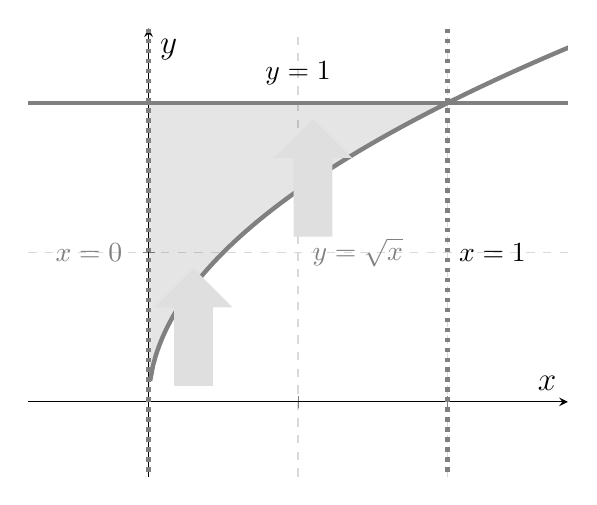
\begin{tikzpicture}
  \begin{axis} [
    Delta Style,
    xmin = -0.25,
    xmax = 1.25,
    ymin = -0.25,
    ymax = 1.25,
    xticklabels = {$ $,$ $,$ $,$ $,$ $,$ $,$ $,$ $,$ $},
    yticklabels = {$ $,$ $,$ $,$ $,$ $,$ $,$ $,$ $,$ $}
    ]

    \addplot[name path=f,domain = 0:1,ultra thin, opacity=1, opacity = 0] {1};

    \addplot[name path=axis, domain = 0:1, ultra thin, opacity=0] ({x^2},{x});

    \addplot [
        thick,
        color=black,
        fill=black,
        fill opacity=0.10
    ]
    fill between[
        of=f and axis,
        soft clip={domain=0:1},
    ];
    
    \addplot [mark=none,ultra thick, gray, samples = 1000] {sqrt(x)};
    \addplot [mark=none, dotted, ultra thick, gray] (0,x);
    \addplot [mark=none, ultra thick, gray] (x,1);
    \addplot [mark=none, dotted, ultra thick, gray] (1,x);
    % \legend{$(\cos x)$,$(\sin x)$,$\cos x \sin x$}
    
    \node[gray] at (axis cs:-0.2,0.5){$x=0$};
    \node[gray] at (axis cs: 0.7,0.5){$y=\sqrt{x}$};
    \node[] at (axis cs: 0.5,1.1){$y=1$};
    \node[] at (axis cs: 1.15,0.5){$x=1$};

    \node[] at (axis cs: 0.55,0.75){\MyArrow[rotate=90]{\phantom{hello}}};
    \node[] at (axis cs: 0.15,0.25){\MyArrow[rotate=90]{\phantom{hello}}};
  \end{axis}
\end{tikzpicture}
\end{document}